\section{Iterações}

Por forma a perceber qual o comportamento da aplicação na infraestrutura que a suporta, aplicou-se o \emph{benchmark} a várias iterações, alterando o número de \emph{Application Servers}, usufruindo da capacidade de escalar horizontalmente esta componente.

Inicialmente procedeu-se a uma otimização da base de dados, como será visto de seguida.

\subsection{Otimização da Base de Dados}

A base de dados é gerada durante o \emph{deployment} da aplicação no servidor aplicacional. Como o \emph{Hibernate} não tem conhecimento da aplicação, não é da responsabilidade do mesmo adicionar índices nem otimizar a base de dados.

A figura seguinte relata os resultados pré-otimização e pós-otimização com dois servidores aplicacionais.

\begin{figure}[ht]
\centerline{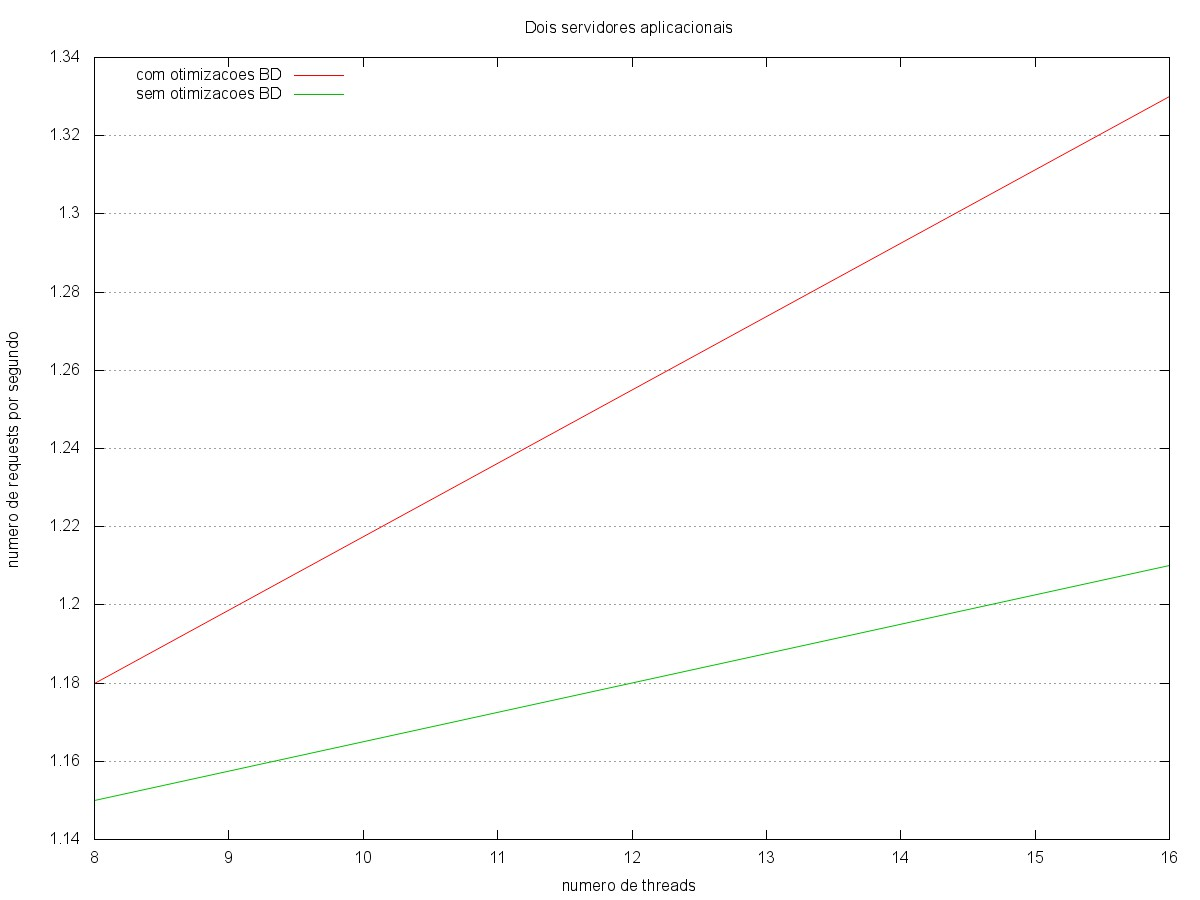
\includegraphics[width=1\textwidth]{images/benchmark/optimization}}
\label{fig:optimization}
\caption{Resultados obtidos antes e depois da otimização}
\end{figure}

Repare que, com otimização, a situação não é tão grave como sem otimização. Para atingir este objetivo, atentou-se nas \emph{queries} efetuadas com mais de \emph{10ms} de tempo de execução, adicionaram-se índices e ordenaram-se algumas tabelas de acordo com alguns deles.

Obtendo-se estes resultados, usou-se a configuração para os testes seguintes.

\subsection{Application Servers}

Prosseguindo os testes com as configurações da base de dados, foi executada a rotina para dois, três e quatro servidores aplicacionais. Não foi executada para mais servidores devido à falta de recursos.

\begin{figure}[ht]
\centerline{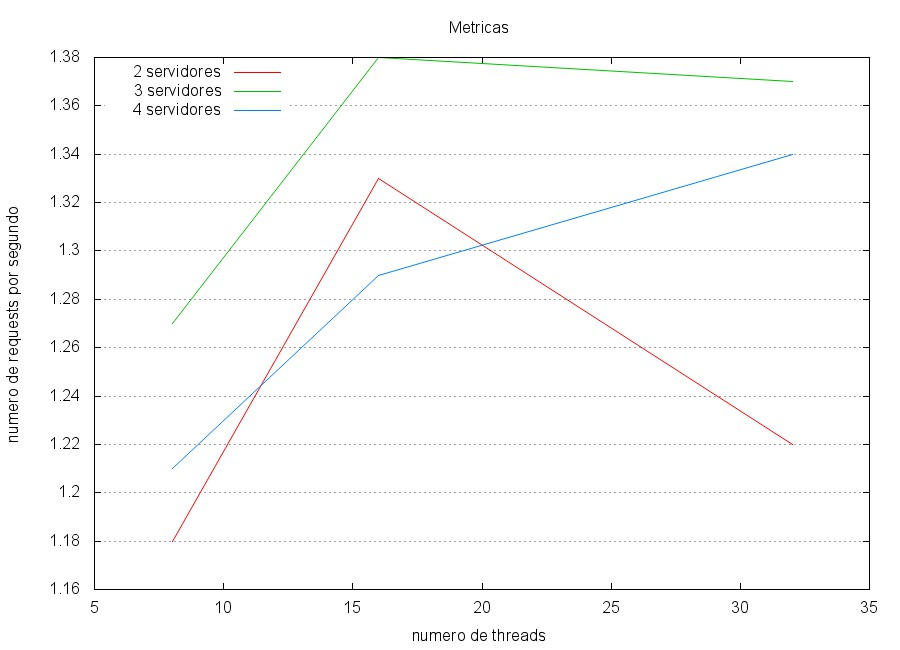
\includegraphics[width=1\textwidth]{images/benchmark/servers}}
\caption{\emph{Benchmark} para dois, três e quatro servidores}
\end{figure}


Como se verifica, a aplicação tem uma grande dificuldade em escalar. O aumento de dois para três servidores aplicacionais resolveu parte do problema, permitindo uma melhoria no desempenho. No entanto, não sendo aquilo que se esperava, adicionar um \emph{Application Server} torna tudo mais lento inicialmente, embora no final do gráfico este continue a crescer. Note, também, que a partir dos 32 clientes o gráfico deixa de existir, devido à falta de recursos para suportar mais do que os referidos. Por acréscimo, as máquinas responsáveis pela \emph{Storage} tiveram um uso de cerca de 30\% de \emph{CPU}.

Tentou-se, também, executar os testes para 64 clientes, mas não se obtiveram resultados, visto que a aplicação atingia o ponto de saturação e o tempo de espera \emph{Apache Bench} alcançava o seu \emph{timeout}.
